%TODO_MAR:  Status: Up for revision

\chapter{Addressing Weakly-coupled Carbon Spins}
Similar to how the electronic spin can be controlled by adding and removing a term to the Hamiltonian we can also control the state of a weakly-coupled carbon-13 atom.
This chapter will start by providing theoretical background on the hyperfine coupling between carbon spins and the NV-center.
The second section will explain how nuclear spins can be addressed.
The next section will explain and show characterization of the nuclear spin environment.
The last section will explain how carbon-spins can be controlled and will demonstrate initialization control and readout of weakly coupled carbon spins.
\section{Hyperfine Coupling}

The Hamiltonian of the nuclear spin depends on the electronic spin state and is given by \cref{eq:carbon_hamiltonian_0} when the electronic-spin is in the $m_s = 0$ state and by \cref{eq:carbon_hamiltonian_1} when in the $m_s = +1$ state for a magnetic field in the z-direction\citep{Taminiau2014Universal}.
 \begin{equation}
 \label{eq:carbon_hamiltonian_0}
H_0= \gamma_{n} B_z I_z
\end{equation}
\begin{equation}
 \label{eq:carbon_hamiltonian_1}
    H_1 = \gamma_{n} B_z I_z +H_{\mathrm{HF}}
\end{equation}
%Replace carbon with nuclear spin (general explanation in revised version of this section).
The Larmor frequency for a carbon nucleus is given by  \cref{eq:carbon_larmor}.
\begin{equation}
\label{eq:carbon_larmor}
\bm{\omega_L} = \gamma_{n}B \bm{\hat{\mathrm{z}}}
\end{equation}

The hyperfine ($H_{\mathrm{HF}}$) term consists of a contact term and a dipole term.
The contact term results from an overlap between the electronic- and carbon- wave-functions making it negligible for all but the carbon-spins closest to the NV-center.
Hyperfine strengths between the NV-center and carbons on close-by lattice sites have been measured\citep{Smeltzer201113} and calculated\citep{Gali2008Ab,Gali2009Identification}, as we are only interested in weakly coupled carbons the contact term of the hyperfine-interaction can be safely neglected.

We define a carbon to be weakly-coupled when its hyperfine coupling strength is much smaller than the Larmor frequency.
For all practical magnetic fields this does not include the close-by carbons that have a contact term in their hyperfine-interaction.
For weakly-coupled carbons the hyperfine-term is equal to the dipole-term and is given by\cref{eq:dipole_component_of_hyperfine}\citep{Lange2012Quantum}.

\begin{equation}
\label{eq:dipole_component_of_hyperfine}
H_{\mathrm{dip}} = \frac{\mu_0 \gamma_e \gamma_{\mathrm{C}} \hbar^2 }{4 \pi r^3} [ \bm{S \cdot I} - 3 (\bm S \cdot \hat{n_{\mathrm{hf}}})(\bm I \cdot \hat{n_{\mathrm{hf}}})]
\end{equation}

From \cref{eq:dipole_component_of_hyperfine}  the parallel and orthogonal components of the Hyperfine interaction, with respect to the NV-axis along the z-direction, can be derived to be:
 \begin{eqnarray}
A_\parallel= - \frac{\mu_0 \gamma_e \gamma_{\mathrm{C}} \hbar^2 }{4 \pi r^3} \left(3\cdot \frac{z^2}{r^2}-1\right)\\
 A_\perp =  -\frac{\mu_0 \gamma_e \gamma_{\mathrm{C}} \hbar^2 }{4 \pi r^3}\left( 3\cdot\frac{\sqrt{x^2+y^2}\cdot z}{r^2}\right)
\end{eqnarray}

Where $H_{\mathrm{HF}} = A_\parallel I_z + A_\perp I_x $.

\section{Addressing Weakly-coupled Carbons through Dynamical Decoupling}
\label{controllingacarbonthroughdynamicaldecoupling}

\begin{figure}[htbp]
\centering
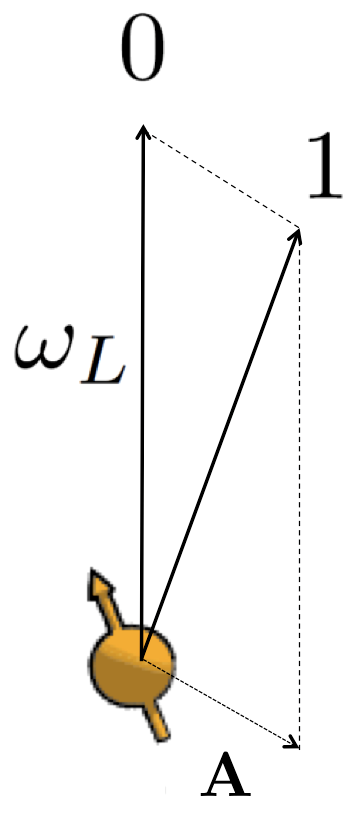
\includegraphics[keepaspectratio,width=0.2\textwidth,height=0.75\textheight]{./img/QuantizationAxis.png}
\caption{Flipping the electron spin from the  $m_s=0$ to the $m_s= +1$ state changes the quantization axis of nuclear spins. For  $m_s=0$ all nuclear spins precess about $\bm{\omega_L}$. For  $m_s=+1$ each spin precesses about a distinct axis $\bm{\tilde{\omega}}=\bm{\omega_L} +\bm{A}$.}
\label{fig:quantax}
\end{figure}

When the electron is in the $m_s=0$ state each nuclear spin precesses about $\bm{\omega_L}$ with the Larmor frequency. When the electron is in the $m_s=+1$ state nuclear spins precess about a distinct axis $\bm{\tilde{\omega}}=\bm{\omega_L} +\bm{A}$ \citep{Taminiau2012Detection}. The hyperfine interaction $\bm{A}$ depends on the position of that particular nuclear spin relative to the NV- center.

When applying a decoupling sequence with N\slash 2 decoupling units of the form {$\tau - \pi -2\tau-\pi-\tau$}, with $\tau$ a wait time between pulses, and $\pi$ a $\pi$-pulse that flips the electron-state, the nuclear spin alternately rotates around the  $\bm\omega_L$ and the $\bm{\tilde{\omega}}$ axis. The net result of one such decoupling sequence is a rotation around an axis $\bm{\hat{\mathrm{n_i}}}$ by an angle $\phi$. Where $\bm{\hat{\mathrm{n_i}}}$ depends on the initial state of the electron: $\bm{\hat{\mathrm{n_0}}}$ when the electron starts in $m_s = 0$ and $\bm{\hat{\mathrm{n_1}}}$ when the electron starts in $m_s = +1$~\citep{Taminiau2012Detection}.

To understand how a carbon-13 atom can be controlled it is useful to consider three situations. In the first situation the $\bm{\omega_L}$ and $\bm{A}$ point in the same direction. In the second situation $\bm{\omega_L}$ and $\bm{A_\perp}$ are of comparable magnitude, resulting in a large angle between the quantization axes. In the last situation $|\bm{A}|$ is small compared to  $\bm{|\omega_L|}$ resulting in a small angle between the quantization axes.

When $\bm{\omega_L}$ and $\bm{A}$ point in the same direction, the net rotation axis is independent of the initial electron-state making it impossible to use the electron to control the carbon-13 atom using this decoupling sequence.

In the case where $\bm{\omega_L}$ and $\bm{A_\perp}$ are of comparable magnitude the net rotation axes $\bm{\hat{\mathrm{n_i}}}$ are strongly dependent on the initial electron-state for almost any $\tau$. This creates entanglement between the electron and this carbon for a wide range of inter pulse-delays $\tau$.

When considering the case where the hyperfine interaction is much smaller than the Larmor frequency ($\omega_L \gg |\bm{A}|$), the net rotation axes  $\hat{n_0}$ and $\hat{n_1}$ are practically parallel and the nuclear spin undergoes an unconditional evolution.
Only when the inter-pulse delay is precisely resonant with the spin dynamics the axes are anti-parallel leading to a conditional rotation\citep{Taminiau2012Detection}.
The resonant condition is given by \cref{eq:res_dip_loc}, where $k$ is an integer and the width of the resonance is given by \cref{eq:res_dip_width}.
% somehow state that resonance gives a dip.
 \begin{equation}
\tau = \frac{(2k+1)\pi}{2 \omega_L + A_\parallel}
\label{eq:res_dip_loc}
\end{equation}

And for $\omega_L \gg |\bm{A}|$ the dip has a width of:

 \begin{equation}
\Delta = \frac{A_\perp}{2 \omega_L^2}
\label{eq:res_dip_width}
\end{equation}

If  $\hat{n_0}$ and $\hat{n_1}$ are not parallel, the resulting conditional rotation of the nuclear spin generally entangles the electron and nuclear spins.

\subsection{Placeholder title for something with intrepreting dd spectroscopy }

As a result, for an unpolarized nuclear spin state, the final electron spin state is a statistical mixture of $|x\rangle$ and $|-x\rangle$ when starting from the $|x\rangle$  state. Where the probability that the initial state is preserved is given by \cref{eq:contrast_to_probability}. The contrast $M_j$ for a single nuclear spin is given by \cref{eq:contrast_single_carbon_spin}\citep{Taminiau2012Detection}.

\begin{equation}
\label{eq:contrast_to_probability}
P_x = (M+1)/2
\end{equation}

\begin{equation}
\label{eq:contrast_single_carbon_spin}
M_j = 1-(1 - \hat{\bm{\mathrm{n_0}}} \cdot \hat{\bm{\mathrm{n_1}}}) \sin^2 \frac{N\phi}{2}
\end{equation}

%alpha = \tilde{\omega} \tau
%beta = (\omega_L \tau)
% mz = (\frac{ A_ \parallel + \omega_L }{ \tilde{ \omega}})
\begin{equation}
\label{eq:vec_term}
    1 - \hat{\bm{\mathrm{n_0}}} \cdot \hat{\bm{\mathrm{n_1}}} =  \frac{A_\perp ^2}{\tilde{\omega^2}} \frac{(1- \cos{(\tilde{\omega} \tau)})(1-\cos{(\omega_L \tau)})} {1 +\cos{(\tilde{\omega} \tau)}\cos{(\omega_L \tau)} - (\frac{ A_ \parallel + \omega_L }{ \tilde{ \omega}}) \sin{(\tilde{\omega} \tau)}\sin{(\omega_L \tau)}}
\end{equation}
\begin{equation}
\label{eq:angle_term}
    \phi =  \cos^{-1}\left(\cos(\tilde{\omega} \tau) \cos(\omega_L \tau)-\left(\frac{ A_ \parallel + \omega_L }{ \tilde{ \omega}}\right) \sin(\tilde{\omega} \tau)\sin(\omega_L \tau)\right)
\end{equation}

\section{Characterizing the Nuclear-spin environment}
% Should add some sort of introduction as to what is in this section
\subsection*{Dynamical Decoupling Spectroscopy}
In reality the electron is not interacting with a single carbon but with a bath of carbon atoms. When the electron interacts with multiple carbons at the same time the contrast $M$ is given by the product of all individual values $M_j$ for each individual spin $j$ (\cref{eq:prod_multiple_spins}). In order to selectively control one carbon the electron should not entangle with any other carbon when addressing it.

\begin{equation}
\label{eq:prod_multiple_spins}
    M = \prod_{j}{M_j}
\end{equation}
%Explain how fingerprint works and how it characterizes how many carbon we can control.
% IF selective, M goes all the way down. If a lot go to 0.5 as all coherence is lost.

To identify promising resonances for carbon control a dynamical decoupling spectroscopy experiment is performed, resulting in a fingerprint of the nuclear-spin environment\citep{Taminiau2012Detection}.
In a dynamical decoupling spectroscopy experiment the electron is prepared in the $|X\rangle = |0\rangle +|1\rangle$ state. It is subjected to a decoupling sequence consisting of N/2 blocks of the form {$\tau - \pi -2\tau-\pi-\tau$}, and concluded by measuring $\langle X\rangle $. The fingerprint is the result of many repetitions for a range of inter-pulse delays $2\tau$.

\subsection*{Contributions of Different Spins }% Needs a better name

A narrow dip in the fingerprint spectrum is an indication of a selectively addressable carbon.
By sweeping the number of $\pi$-pulses on such a dip it can be verified if it corresponds to a \emph{single} carbon.
If entanglement is created with a lot of spins at once all coherence is lost and contrast will go to 0.
Only if no entanglement is created with other carbons can the contrast be sweeped to -1. %This weird wording is used because it is possible that the response of another carbon is non existent exactly when the first one reaches -1. Maybe also add the in between case for few spins?

Because carbon-13 atoms are randomly distributed in diamond there is a wide range of possible hyperfine strengths.
Most carbon-spins have very similar hyperfine-interaction strengths as they are relatively far away from the NV-center. This causes their resonances to overlap, manifesting itself as a broad feature with little coherence in the fingerprint. We identify this response as the spin-bath collapse.
% reality most far away -> similar strengths ->  spin bath response

Spins that have a stronger than average hyperfine-interaction show up outside or at the edge of the spin-bath collapse. Going to larger $\tau$ separates resonances further as their order $k$ increases, allowing for control of more spins.
 As computations are fundamentally limited by the coherence time there is a limit to the resonance-order that can be used to address carbons.

  Some of the relatively strong-coupled spins have a strong orthogonal-component of the hyperfine interaction. This orthogonal-component causes a broad response, effectively blocking a large range of $\tau$ from being used to control other spins.

\subsection*{Effect of the magnetic field}
% need the stronger
% sometimes one that is to strong -> increase B-field
Both these issues can be alleviated by increasing the magnetic field.
By increasing the magnetic field the Larmor frequency can be made much larger than the orthogonal components of the hyperfine interactions causing the broad resonances to disappear, allowing more carbon resonances to be selectively addressed.
% until the orthogonal hyperfine-components of all spins are small relative to the Larmor frequency the broad resonances that cause large parts of the spectrum to become useless disappear.
% Additionally increasing the magnetic field causes resonances to move closer to $\tau =0$ (\cref{eq:res_dip_loc}), while at the same time becoming narrower (\cref{eq:res_dip_width}), allowing higher order resonances to be addressed within the same time-window. % use calculations of Tim to show that number of resonances that can be addressed increases linearly with magnetic field.

% to much B-field -> to narrow dips, cannot address anymore (tech limitation)
Increasing the magnetic field will not always improve the situation. When the magnetic field is too strong the resonances become narrower than the resolution of the Arbitrary Waveform Generator used to generate the pulses that address the resonances, making it impossible to address these resonances effectively.
Simulations that were performed (see \cref{chap:addressable_carbon_sims}) indicate that for diamond with a natural concentration of carbon-13 there is a broad range between 400G and 1400G where the magnetic field is optimal.

There are also practical limitations to how much the magnetic field can be increased. In order to control carbon-spins we must still be able to coherently initialize, control and read-out the electronic-spin-state. Because the transitions used for read-out and initialization depend on strain and magnetic field\citep{Hensen2011MeasurementBased}, care must be taken when measuring at different magnetic fields that states do not mix in the excited state.
This combined with the fact that few experiments have been performed at high magnetic field and low temperature make it more practical to settle for a more moderate magnetic field of 300G.
%Still misses point not practical to compensate for extremely strongly coupled spins.
% Optimum B-field range 300-700
%sims indicate optimum B? of behouden voor appendix?
% Additional problems with B. Stability? -> appendix. transitions in excited states?


\subsection*{Identifying Individual Carbon-spins}
To identify spins a dynamical decoupling spectroscopy was performed on the sample with N = 8, 16, 32 and 64 pulses. For N =8, 16 and 32 pulses this was done between $\tau = 2 \mu \mathrm{s}$  and $72 \mu \mathrm{s}$ and for N = 64 this was done up to $\tau = 52 \mu \mathrm{s}$.
We identify distinct features in the fingerprint and try to assign different hyperfine-couplings to them such that the computed data for these spins fits the measured data as well as possible.
The response of a single spin is computed using \cref{eq:contrast_single_carbon_spin}.
13 spins were identified using this method.

\Cref{fig:FP} shows a subset of the fingerprint data acquired for this thesis. \Cref{tbl:HF_par} shows the estimated hyperfine parameters of the 4 carbon spins with the strongest coupling.
All estimated hyperfine parameters and a link to the full fingerprint measurements can be found in \cref{chap:Fingerprint_data_appendix}.

The broad collapse due to the spin bath is clearly visible at $\tau/(4 \tau _L)$ for odd $m$, with $m \in \mathbb{N}$ .
The most prevalent feature of the spectrum is a strong oscillation between the spin-bath collapses.
This oscillation can be explained by a single carbon that has a strong orthogonal hyperfine coupling, labeled spin-2 in our analysis.
Due to the nature of spin-2 it is hard to find other carbons that can be coherently controlled.

Nonetheless there are still some distinct peaks at the edge of the spin-bath collapse. When going to higher orders we see these peaks separate from the spin-bath response.
We find that we can address 4 spins.
These are listed in \cref{tbl:HF_par}. % Remove this sentence?


% Table with T2*, HF_parr, HF_orth. Values can be found in QEC LT/Simulations/Hans_Sil01_Spin_Control
% B_field = 304.22G
\begin{figure}[htbp]

    \begin{subfigure}[t]{\textwidth}\centering
        \centering
        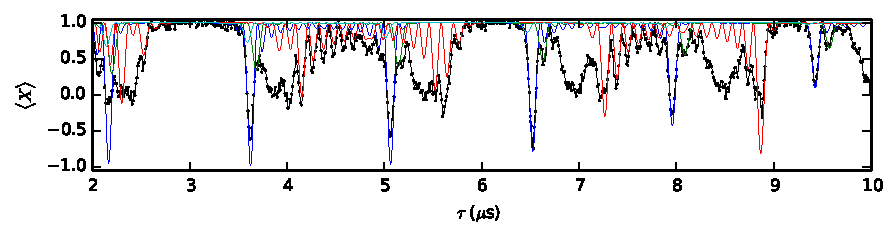
\includegraphics{Img/fingerprint16.pdf}
        %TODO_MAR: use annotations to add labels in the graphs using matplotlib
        \caption{Fingerprint for N=16 pulses. }
        \label{fig:FP16}
    \end{subfigure}

    \begin{subfigure}[t]{\textwidth}\centering
        \centering
        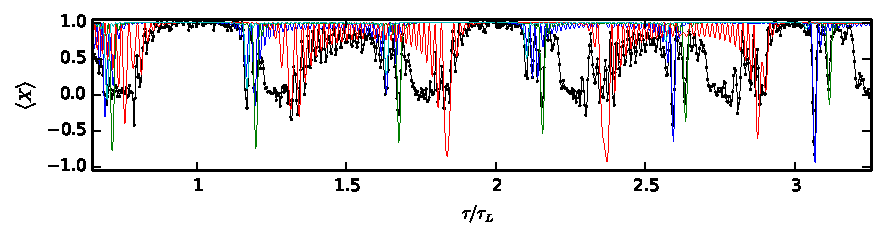
\includegraphics{Img/fingerprint32.pdf}
        %TODO_MAR: use annotations to add labels in the graphs using matplotlib
        \caption{Fingerprint for N =32 pulses. }
        \label{fig:FP32}
    \end{subfigure}
    \caption{Part of a fingerprint resulting from a dynamical-decoupling-spectroscopy experiment performed at 304.12G. A reference to the full spectroscopy can be found in \cref{chap:Fingerprint_data_appendix}.  Colored lines represent computed responses of carbon spins. Responses were calculated using \cref{eq:contrast_single_carbon_spin} with hyperfine parameters from \cref{tbl:HF_par}. NOTE: labels for colored spins still coming. }
    \label{fig:FP}
\end{figure}


\begin{table}[htbp]
    \begin{tabular}{cllll}
    Carbon & \quad \quad  $A_{\parallel} $ & \quad \quad $A_{\perp}$ \\ \hline
    1         & $2 \pi \cdot${ }30.0 kHz             & $2 \pi \cdot${ }80.0 kHz                \\
    2         & $2 \pi \cdot${ }27.0 kHz             & $2 \pi \cdot${ }28.5 kHz              \\
    3         & $2 \pi \cdot$-51.0 kHz          & $2 \pi \cdot$105.0 kHz              \\
    4         & $2 \pi \cdot${ }45.1 kHz           & $2 \pi \cdot${ }20.0 kHz                \\
    \end{tabular}
    \caption{Estimated hyperfine parameters for spins 1 to 4 in \cref{fig:FP}.}
    \label{tbl:HF_par}
\end{table}
